\documentclass[conference]{IEEEtran}

\usepackage[utf8]{inputenc}
\usepackage[T1]{fontenc}
\usepackage[czech]{babel}
\usepackage{cite}
\usepackage{amsmath,amssymb,amsfonts}
\usepackage{booktabs}
\usepackage{tabularx}
\usepackage{graphicx}
\usepackage{textcomp}
\usepackage{xcolor}
\usepackage{url}

\newcommand{\code}[1]{\texttt{#1}}
\newcolumntype{Y}{>{\raggedright\arraybackslash}X}
\newcommand{\placeholder}[1]{%
  \fbox{%
    \begin{minipage}{0.92\linewidth}
      \centering\small #1
    \end{minipage}%
  }%
}

\begin{document}

\title{Akustická lokalizace dronu mikrofonním polem 2$\times$8 na mikrokontroléru STM32H563}

\author{\IEEEauthorblockN{Martin Maxa}
\IEEEauthorblockA{CTU, FEE\\
Prague, Czechia\\
maxamart@fel.cvut.cz}}

\maketitle

\begin{abstract}
% TODO M5: abstrakt az po vysledcich simulace.
\placeholder{Abstrakt doplnit v~milníku M5.}
\end{abstract}

\begin{IEEEkeywords}
beamforming, direction of arrival, SRP-PHAT, mikrofonní pole, drone acoustics
\end{IEEEkeywords}

\section{Úvod}
Akustická detekce dronu odpovídá na otázku, zda je dron v~okolí uzlu přítomen. Pro navazující reakci je užitečné znát také směr, ze kterého jeho zvuk přichází. Lokalizaci lze od detekce oddělit. Detektor běží nepřetržitě a~uzel přitom drží krátkou historii vícekanálového signálu. Teprve po spuštění detektoru se nad uloženým úsekem odhadne směr příchodu zvuku (direction of arrival, DOA). Výpočetně náročná prostorová analýza tak probíhá jen ve chvíli, kdy má smysl.

Cílem práce je připravit podklady pro mikrofonní pole se dvěma kruhy po osmi mikrofonech, připojené k~mikrokontroléru STM32H563. Práce shrnuje metody beamformingu a~odhadu DOA, z~frekvenční struktury dronového hluku odvozuje pracovní pásmo, simulací porovnává varianty geometrie pole a~odhaduje paměťové a~výpočetní nároky lokalizace na cílovém mikrokontroléru.

\section{Beamforming a odhad směru příchodu}
\label{sec:sota}
% TODO M2: far-field model a steering vektor, TDOA, prostorovy aliasing,
% DAS/SRP, MVDR (Capon), GCC-PHAT (Knapp & Carter), SRP-PHAT (DiBiase),
% MUSIC (Schmidt), TOPS, UCA vs 3D pole, aktualni prace o lokalizaci UAV.
\placeholder{Přehled metod beamformingu a~DOA doplnit v~milníku M2.}

\section{Spektrum dronového hluku}
\label{sec:spektrum}
Frekvenční strukturu dronového hluku jsme převzali z~analýzy datasetu DADS (Drone Audio Detection Samples) \cite{basso2024dads}. Dataset obsahuje 163\,591 dronových a~16\,729 ne-dronových nahrávek. Všechny mají vzorkovací kmitočet 16\,kHz, 16bitové vzorky a~jeden kanál. Pro každou nahrávku byla výkonová spektrální hustota (PSD) spočtena Welchovou metodou s~oknem 2048 vzorků a~50\% překryvem a~spektra byla zprůměrována v~lineárním výkonovém měřítku (obr.~\ref{fig:dads_spectrum}).

Dronový pohon vytváří tóny na frekvenci průchodu listů vrtule $f_{\mathrm{BPF}}=N_b f_r$, kde $N_b$ je počet listů a~$f_r$ otáčková frekvence, a~jejich harmonické násobky. U~malých UAV se dvěma až čtyřmi listy a~otáčkami 3\,000 až 9\,000~min$^{-1}$ leží BPF přibližně mezi 100 a~600\,Hz. Pod 1\,kHz mají dronové nahrávky průměrnou PSD o~10 až 15\,dB vyšší než nahrávky bez dronu, nad 1\,kHz se průměry obou tříd přibližují.

Pro lokalizaci z~toho plyne, že většina energie dronu, a~tedy i~využitelné prostorové informace, leží pod 1 až 2\,kHz. Toto pásmo je pod hranicí prostorového aliasingu uvažovaných polí o~průměru 160 a~200\,mm (tab.~\ref{tab:alias}). Beamforming proto stačí počítat jen ve vybraných frekvenčních binech přibližně mezi 300\,Hz a~2\,kHz. Nahrávky DADS zároveň slouží jako zdrojový signál simulace v~sekci~\ref{sec:geometrie}.

\begin{figure}[t]
  \centering
  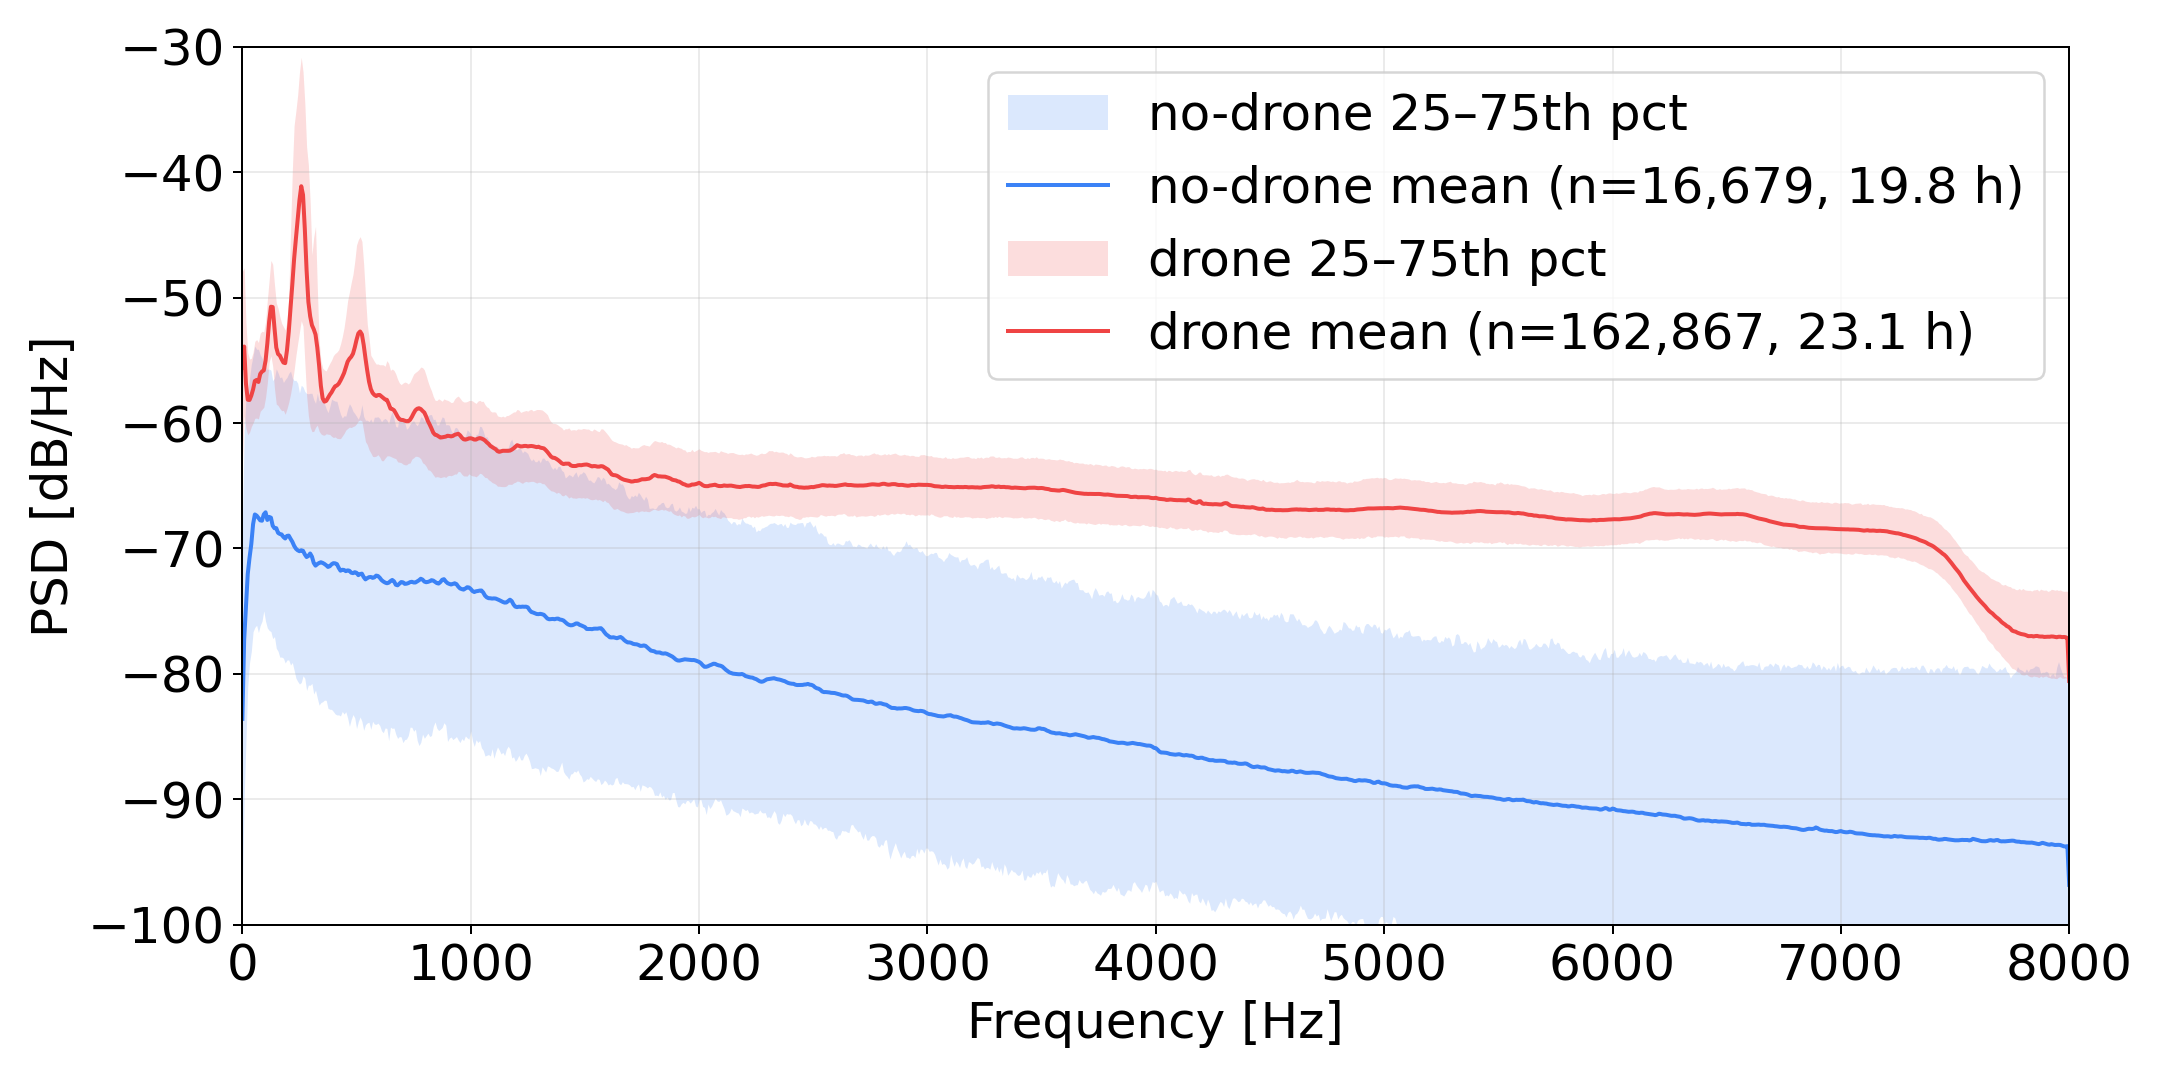
\includegraphics[width=\columnwidth]{figures/dads_average_spectrum.png}
  \caption{Střední PSD pro dronové ($n=163\,591$, červeně) a~ne-dronové ($n=14\,868$, modře) nahrávky z~datasetu DADS. Pásma odpovídají 25.–75.~percentilu přes nahrávky.}
  \label{fig:dads_spectrum}
\end{figure}

\section{Geometrie mikrofonního pole}
\label{sec:geometrie}
% TODO M4: vysledky sweepu, doporucena geometrie pro PCB a doporucena metoda.
% Topologie: 1x8 kruh, 2x8 kruhy nad sebou, 2x8 kruhy pootocene o 22,5 st.
% Prumer 160/200/250 mm, rozteč kruhu h 40/70/100 mm.
% Signal: DADS, free-field zpozdeni do 16 mikrofonu, aditivni sum, sweep SNR.
% Metriky: RMSE azimutu a elevace vs SNR, sirka hlavniho laloku, vypocetni cena.
\placeholder{Simulace a~volbu geometrie doplnit v~milníku M4.}

\section{Hardware}
\label{sec:hw}
\begin{itemize}
  \item \textbf{Převodník PDM$\rightarrow$TDM:} ADAU7118 \cite{adiadau7118}. Převádí osm PDM kanálů ze čtyř stereo datových linek na jeden PCM stream I$^2$S nebo TDM (až TDM16). Sériové rozhraní pracuje jako slave, $f_s$ je 4 až 192\,kHz a~BCLK může být 64$\times$ až 512$\times f_s$. Dvě výstupní PDM hodiny pro mikrofony generuje automaticky. V~hardwarovém módu bez I$^2$C podporuje jen TDM, takže deska pole nepotřebuje konfigurační MCU. Pouzdro LFCSP-16 má rozměry 3$\times$3\,mm.
  \item \textbf{Zapojení:} každý kruh tvoří samostatnou desku s~osmi PDM MEMS mikrofony a~jedním ADAU7118, který dává jeden stream TDM8. Dvě identické desky jsou nad sebou na distančních sloupcích. SAI1 blok A pracuje jako master přijímač: generuje BCLK a~FSYNC a~čte data první desky. Blok B je k~němu synchronní slave a~čte data druhé desky. Kabelem tedy vedou čtyři signály (BCLK, FSYNC, SD\_A, SD\_B) a~napájení.
  \item \textbf{Hodiny:} TDM8 s~32bitovými sloty při $f_s=48$\,kHz vyžaduje BCLK 12{,}288\,MHz, tedy $256 f_s$, což je v~povoleném rozsahu ADAU7118. Stejný kmitočet už dnes generuje PLL2 pro SAI1 ve firmwaru uzlu.
  \item \textbf{Úprava uzlu:} deska uzlu v0.1 vede na konektor FFC J11 piny PE2, PE4, PE6 a~PF10 (dnes PDM CK1, D2, D1, D3). Žádný z~nich nemá funkci SAI SCK, proto TDM na v0.1 nelze použít. Revize v0.2 musí přepojit PE2 na PE5 (SAI1\_SCK\_A) a~PF10 na PE3 (SAI1\_SD\_B). PE4 (FS\_A) a~PE6 (SD\_A) zůstávají a~konektor J11 se nemění.
\end{itemize}

\section{Výpočty a vztahy}
\label{sec:vypocty}
\subsection*{Datový tok a hodiny}
Akvizice 16 kanálů při $f_s=48$\,kHz s~32bitovými sloty dává datový tok
\begin{equation}
  R = M f_s w = 16 \cdot 48\,000 \cdot 4\,\mathrm{B} \approx 3{,}07\,\mathrm{MB/s},
\end{equation}
po uložení jako 16bitové vzorky 1{,}54\,MB/s. Bitová hodina jednoho streamu TDM8 je
\begin{equation}
  f_{\mathrm{BCLK}} = f_s N_{\mathrm{slot}} w_{\mathrm{slot}} = 48\,000 \cdot 8 \cdot 32 = 12{,}288\,\mathrm{MHz}.
\end{equation}

\subsection*{Lokalizační buffer}
Po spuštění detektoru se vezme úsek $T=100$\,ms, filtrem dolní propusti a~decimací 3:1 se převede z~48 na 16\,kHz a~uloží jako 16bitové vzorky. Na kanál připadá $N = f_s' T = 1600$ vzorků a~celý úsek zabere
\begin{equation}
  16 \cdot 1600 \cdot 2\,\mathrm{B} = 51{,}2\,\mathrm{kB},
\end{equation}
což je malý zlomek 640\,kB SRAM mikrokontroléru STM32H563.

\subsection*{Prostorový aliasing}
Pro $M_r$ mikrofonů rovnoměrně na kružnici o~poloměru $r$ je vzdálenost sousedů a~přibližná horní mez bez aliasingu
\begin{equation}
  d = 2r\sin\frac{\pi}{M_r}, \qquad f_{\mathrm{alias}} = \frac{c}{2d},
\end{equation}
kde $c=343$\,m/s. Pro svislou rozteč kruhů $h$ platí obdobně $f_{\mathrm{alias}} = c/(2h)$. Hodnoty pro uvažované rozměry shrnuje tab.~\ref{tab:alias}.

\begin{table}[t]
\centering
\caption{Mez prostorového aliasingu pro $M_r=8$ a~uvažované rozměry}
\label{tab:alias}
\begin{tabular}{@{}lrr@{}}
\toprule
Rozměr & $d$ [mm] & $f_{\mathrm{alias}}$ [kHz] \\
\midrule
$\varnothing$\,160\,mm & 61{,}2 & 2{,}80 \\
$\varnothing$\,200\,mm & 76{,}5 & 2{,}24 \\
$\varnothing$\,250\,mm & 95{,}7 & 1{,}79 \\
\midrule
$h=40$\,mm & 40{,}0 & 4{,}29 \\
$h=70$\,mm & 70{,}0 & 2{,}45 \\
$h=100$\,mm & 100{,}0 & 1{,}72 \\
\bottomrule
\end{tabular}
\end{table}

\subsection*{STFT a směrový grid}
Úsek 1600 vzorků se dělí na rámce $N_{\mathrm{FFT}}=512$ (32\,ms při 16\,kHz) s~50\% překryvem, což dává 5 rámců s~frekvenčním rozlišením 31{,}25\,Hz. Pásmu 300\,Hz až 2\,kHz odpovídají biny 10 až 64, tedy 55 binů.

Hrubý grid s~krokem 5$^\circ$ přes azimut 0 až 355$^\circ$ a~elevaci 0 až 90$^\circ$ má $72 \cdot 19 = 1368$ směrů, jemný grid s~krokem 1$^\circ$ by jich měl $360 \cdot 91 = 32\,760$. Proto se nejdřív prohledá hrubý grid a~jemně se dohledává jen okolí maxima. Tabulka zpoždění $\tau_m = \mathbf{r}_m\cdot\mathbf{u}(\phi,\theta)/c$ ve formátu float32 zabere pro hrubý grid $16 \cdot 1368 \cdot 4\,\mathrm{B} \approx 87{,}6$\,kB, kdežto pro grid 1$^\circ$ asi 2{,}1\,MB, tedy celou interní Flash.

% TODO M5: pocet operaci zvolene metody (FFT 16 kanalu x 5 ramcu,
% 55 binu x 1368 smeru x 16 mikrofonu) a odhad casu na 250 MHz Cortex-M33.

\bibliographystyle{IEEEtran}
\bibliography{references}

\end{document}
